\section{Interfacing with Applications}

\ken{
  Each subsection should be up to 2/3 pages plus have images up to 1/2 page.
  (3.5 pages total.)
  The section should start with a layperson overview of what the domain problem is, what scientists are doing to study the problem.
  The section should then explain how visualization fits in to help.
  Explain the technical solution of how VTK-m was integrated into the system and describe the final result.
  The section may repeat for multiple things that were done.
  For example the fusion reactor could first talk about in situ images and then Poincar\'{e} plots.
  The laser wakefields could talk about deliver of in situ images via Ascent and then about the customized particle advection.
  The final section will be a little different in that it will iterate over multiple science domains.
}

\subsection{Tokamak Fusion Reactor}

\assign{Dave}

(WDMApp/CS Chang/Poincar\'{e})

\subsection{Laser Wakefield Acceleration}

\assign{Axel, Abhi}

%\defcitealias{FedeliHuebl2022}{Fedeli, Huebl et al. (2022)}
%\citepalias{FedeliHuebl2022}

WarpX is a new particle-in-cell simulation code developed as part of ECP, which was awarded the 2022 ACM Gordon Bell Prize~\cite{FedeliHuebl2022}.
Science case ...3

WarpX coarse parallelization relies on block-structured domain-decomposition with MPI using the AMReX library~\cite{} and compute acceleration with CUDA/HIP/SYCL or OpenMP, so that simulations are scalable to the world's largest supercomputers.

If WarpX would rely on traditional post-processing workflows alone for visualization of the dynamics of Exascale simulations, the resulting multi-PByte scale output would severely limit the available snapshots or level of detail to visualize.
Consequently, integrations with ...

\begin{figure}[htb]
  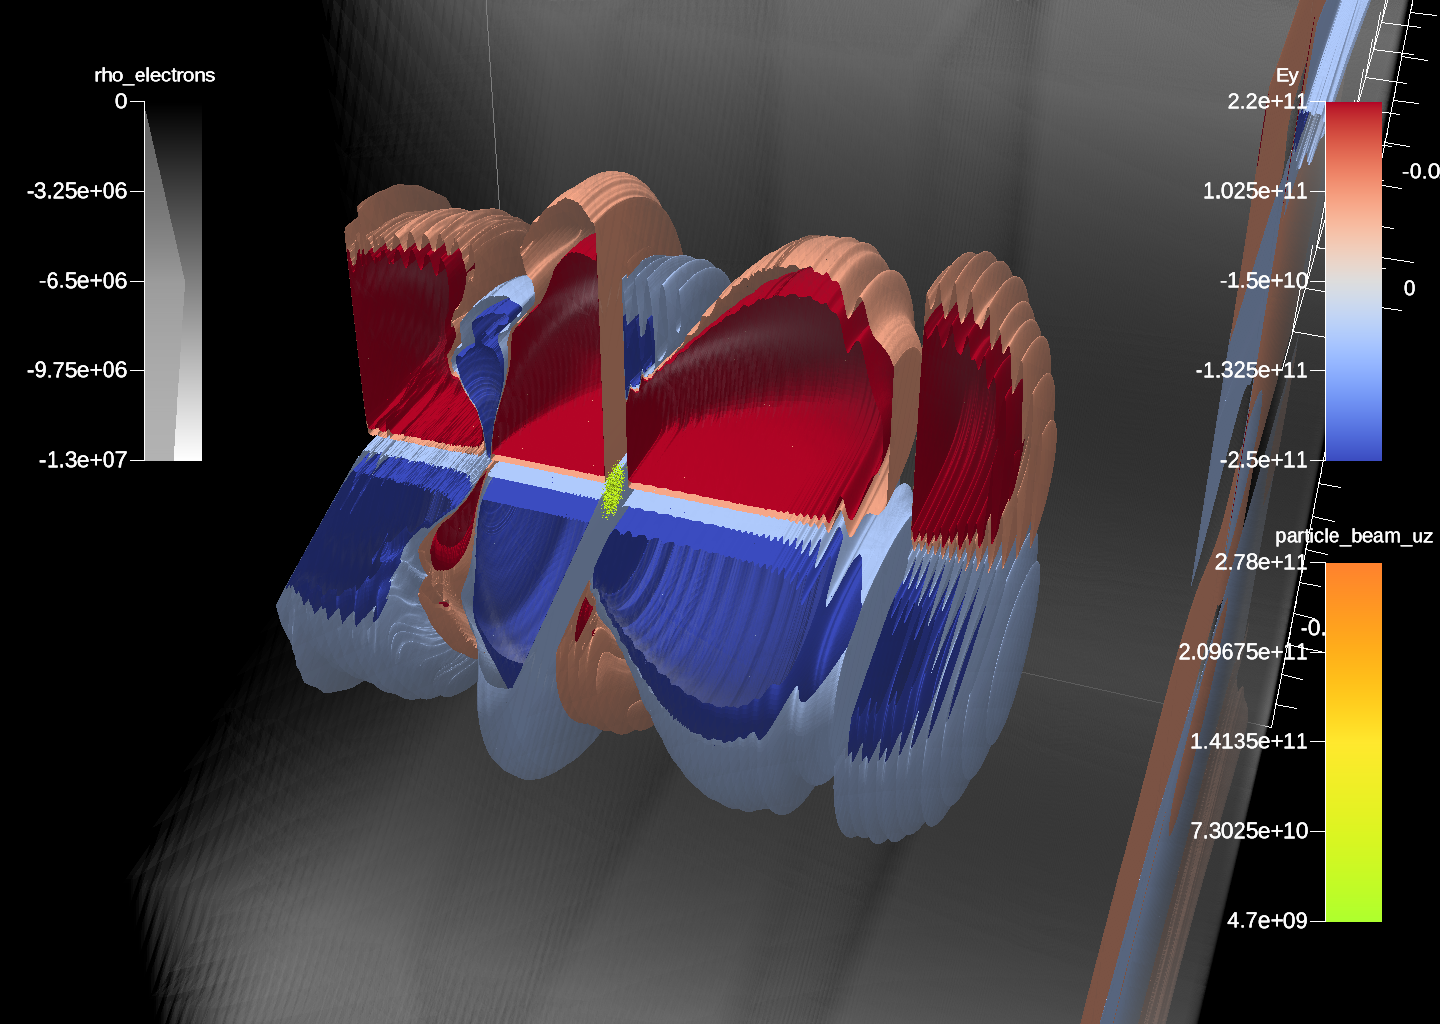
\includegraphics[width=\linewidth]{figures/warpx_stages_lwfa.png}
  \caption{WarpX in situ visualization on 552 Frontier GPUs using Ascent and VTK-m.}
  \label{fig:warpx_lwfa}
\end{figure}

Custom particle advection algorithm in VTK-m: ...

\subsection{Impact Beyond ECP}

\assign{Jay}

%\jay{discuss the applications/use cases outside of ECP}
In addition to the applications mentioned above, VTK-m still serves as the key infrastructure for accelerating data analysis and visualization in various scientific applications through \emph{in situ} approach. This subsection lists several typical examples and illustrates how VTK-m is integrated into \emph{in situ} scientific workflows outside of ECP.


Before being selected as a project in ECP, VTK-m was a core component in Visualization for the Extreme-Scale Scientific Computation Ecosystem (XVis)~\cite{Moreland2019}. 
XVis focused on multiple ways to integrate \emph{in situ} visualization with the simulation, extract key information, and decrease the data size for post-hoc processing.
The ``\emph{in situ} reduction + post hoc'' paradigm is widely adopted in multiple scientific domains, such as probability distribution functions (PDF) extraction of fields in combustion simulation~\cite{7874311}, and binning mechanism to reduce the data size of fusion simulation~\cite{Kress2018}. 


Nyx is a cosmological simulation that aims to solve compressible hydrodynamics with N-body treatment of the dark matter. Each simulation run may contain hundreds of time steps with multiple sets of simulation input parameters. The raw data size is usually hundreds of TBs to several PBs, which causes challenges to process data in post-processing. 
VTK-m is used as \emph{in situ} analysis to extract the statistical properties of the down-sampled data to hugely reduce the size of raw data. The associated statistics model can be used to construct the data based on prior knowledge in post-processing with low data reconstruction error~\cite{Wang2019}.

Eddy detection and tracking plays a key role in the ocean simulation field. Understanding the characteristics of eddies can help scientists to explain the regional air-sea interactions.
VTK-m streamline filter can be used as an \emph{in situ} analysis to generate streamline data used for interactive post-hoc analysis~\cite{Han2022}. With the help of VTK-m, the associated eddy analysis workflow can improve the interaction speed, reduce data storage, and meet the
needs of real-time visual analysis interaction.  
